\documentclass[11pt]{article}
\usepackage[a4paper, margin=20mm]{geometry}
\usepackage{wrapfig}
\usepackage{jtygm}
\usepackage{listings}
\usepackage[usenames, dvipsnames]{color}
\usepackage[dvipdfmx]{graphicx}
\usepackage{keystroke}
\usepackage{menukeys}
\usepackage{siunitx}

\newcommand\gamename{SamurAI Jockey}

\title{{\gamename} Game Rule (draft)}
\author{IPSJ Programming Contest Committee}
\date{2017/09/16}

\begin{document}
\maketitle

\begin{abstract}
  A draft version of the game rule for SamurAI Coding 2017--2018.
  Note that this is a draft and is subject to change.
\end{abstract}

\section{Game Outline}
Two players controlled by AI programs, changing their positions step
by step, compete for time to goal in a course with obstacles.

One game consists of two races with the same course, exchanging the
start positions of two players.
The player with the smaller sum of goal times of two races wins the game.
If the goal time sums are equal, the game is a draw.

\begin{wrapfigure}{r}{0.38\columnwidth}
  \vspace{-2cm}
  \centering
  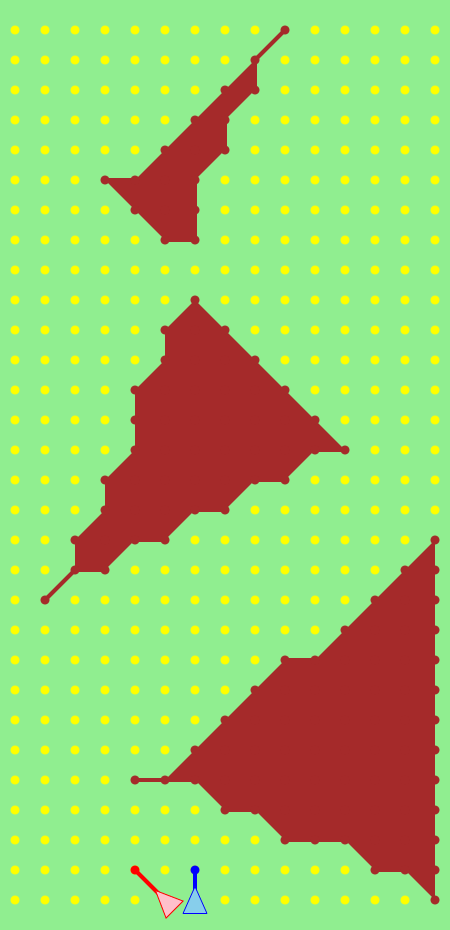
\includegraphics[width=0.35\columnwidth, natwidth=450, natheight=930]{racecourse.png}
  \caption{Race Course Example}
  \label{fig:course}
\end{wrapfigure}

\section{Race Course}
The race courses are a two dimensional grid, with different sizes and
obstacle positions for different games.  The width of the race course is
$w$ and its length is $l$ in what follows.  A grid point on the race
course has coordinates $(x,y)$ ($0\le x < w, 0\le y$).

Some of the grid points on the race course are {\em obstacle points.}
Obstacle points and line segments connecting them are {\em obstacles.}
Obstacles are fixed in one race.  The AI programs controlling players
(called {\em AI,} in what follows), however, are given information of
only those obstacles inside the players' fields of vision, that is,
those with their $y$-coordinates within a certain limit from the
$y$-coordinates of the players' positions.  As only limited
acceleration and deceleration are possible, obstacles may become
unavoidable with velocity too large.

Figure \ref{fig:course} shows an example of a race course.  The brown
dots are obstacle points, brown line segments are obstacles connecting
obstacle points, and the brown areas are those surrounded by obstacles
into which players cannot enter.

During one race, two players are on different grid points.  The start
points of two players are with $y$-coordinates of $0$ and different
$x$-coordinates.  As the race progresses, players change their
positions step by step.  Players finish the race when they have reached
a point with the $y$-coordinate greater than or equal to the course
length $l$.

There is never a dead end in the course.  A player can move from any
grid points of the race course to a point with larger $y$-coordinate,
never decreasing its $y$-coordinate during the move, if moves are with
velocity small enough.

\section{Race Process}
On every step of a race, both AI's are given information on the race
situation, and the situation is updated according to the
acceleration/deceleration instruction given by the players in
response.  Two players never occupy the same position at a time during
a race.

The race starts from step 0 and the step number is incremented one by
one.  The race ends when both of the players finish.  If one or more
players can't finish within the step limit, however, the race ends at
that step.  The goal time of the unfinished player is twice the step
limit.

\subsection{Time Control}
A limit is imposed on the total of time a player can use in one race.
The clock starts or resumes when the game manager program has finished
sending information to the player AI and stops when it has finished
receiving the response from the player AI.  The player running out of
the time loses the game including the race.
\footnote{The time limit is not fixed yet but is expected to be some
  tens of seconds.}

\subsection{Player States and Acceleration Instructions}
A player has its {\em position} $(x, y)$ and {\em velocity} $(v_{\rm
  x}, v_{\rm y})$ at each step.

A player instructs {\em acceleration|} $(a_{\rm x}, a_{\rm y})$ at each step.
Both $a_{\rm x}$ and $a_{\rm y}$ should be one of $-1, 0,$ or $1.$

When the player can make normal move without committing course out and
collision with the opponent without priority (described below), the
position of the player at the next step will be $(x+v_{\rm x}+a_{\rm
  x}, y+v_{\rm y}+a_{\rm y})$.  This position is called the {\em
  planned position} in what follows.  The velocity of the player in
the next step will be $(v_{\rm x}+a_{\rm x}, v_{\rm y}+a_{\rm y})$
whether or not the player can make normal move.

\begin{wrapfigure}{R}{0.28\columnwidth}
  \vspace{-1cm}
  \centering
  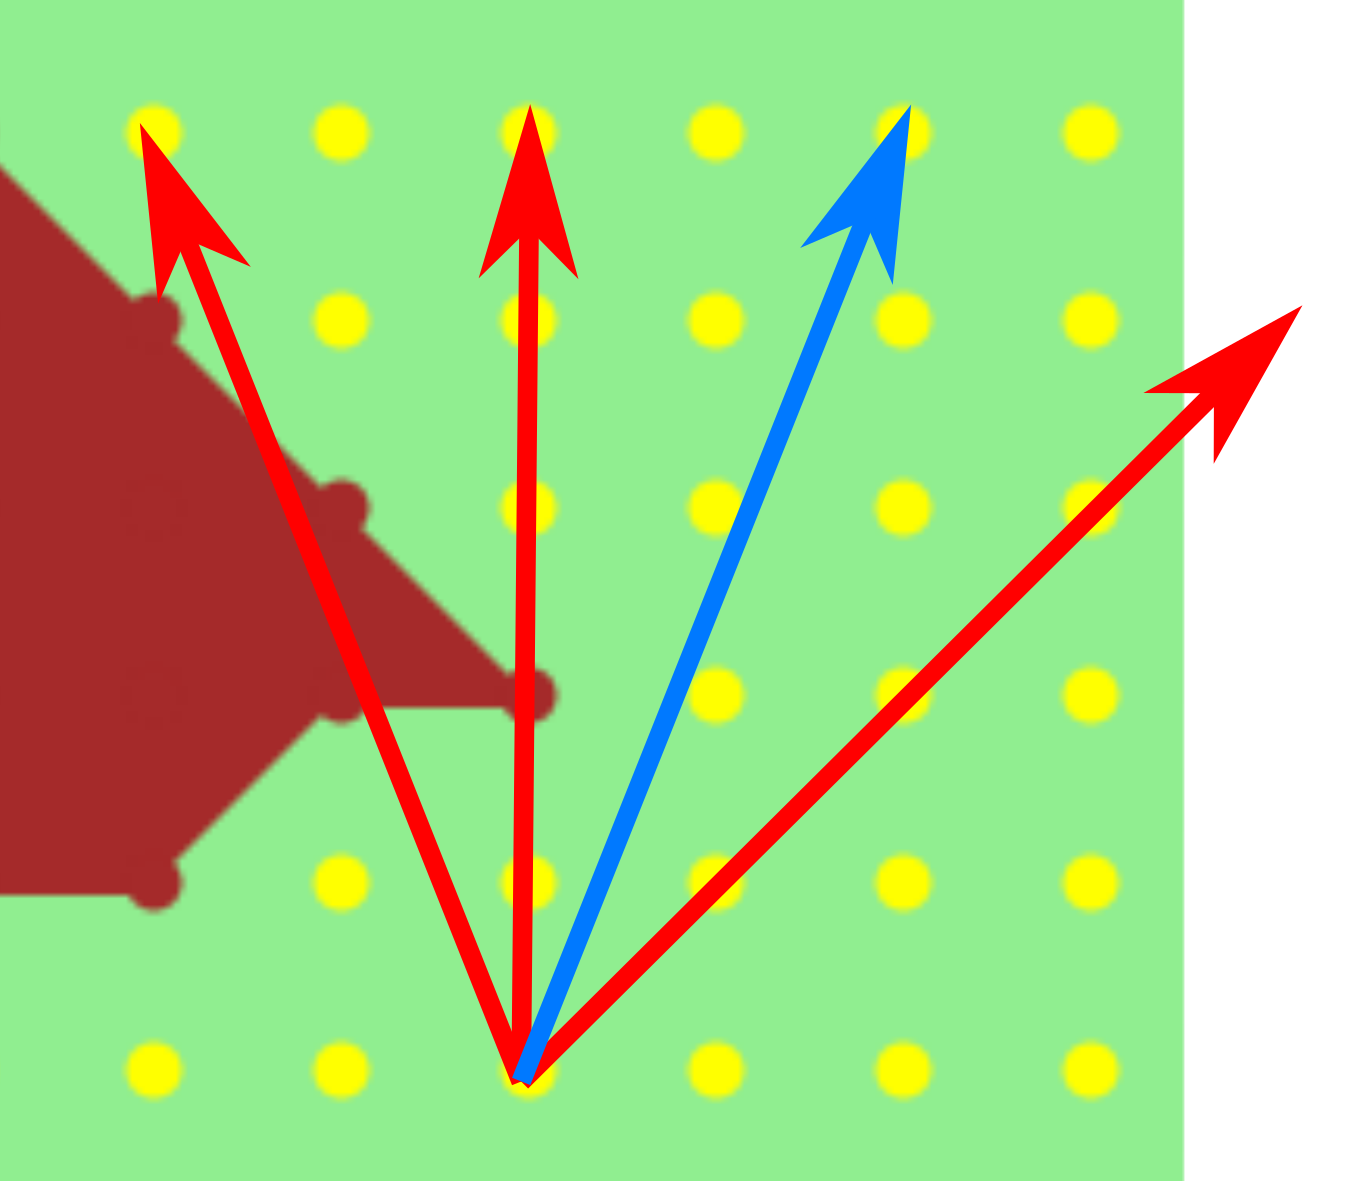
\includegraphics[width=0.26\columnwidth, natwidth=1358, natheight=1181]{courseout.png}
  \caption{Course Outs}
  \label{fig:courseout}
  Red movement lines cause course outs.
  \vspace{-1cm}
\end{wrapfigure}

\subsection{Movement Lines and Course Outs}
The line segment connecting the players position and its planned position is called the {\em movement line} of the player.

The player commits a {\em course out} if one or more of the
following hold.
\begin{itemize}
\item
  The player goes out of the course, that is, the coordinates of
  planned position $(x, y)$ does not satisfy both $0\le x<w$ and $0\le
  y.$
\item
  The movement line goes over or touches one or more obstacles.
\end{itemize}

The position of a player that committed a course out cannot move: its
position in the next step remains the same.  The acceleration is
applied the same as when no course outs are committed.

\begin{wrapfigure}{R}{0.32\columnwidth}
  \centering
  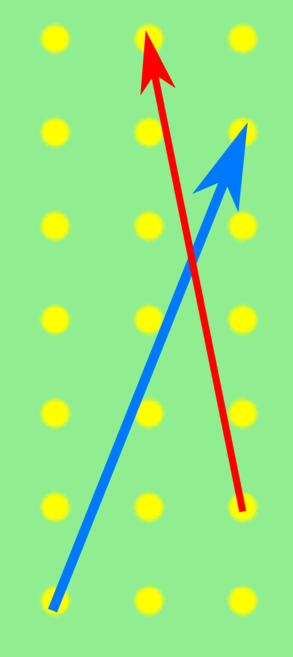
\includegraphics[scale=0.2, natwidth=293, natheight=657]{collision.png}
  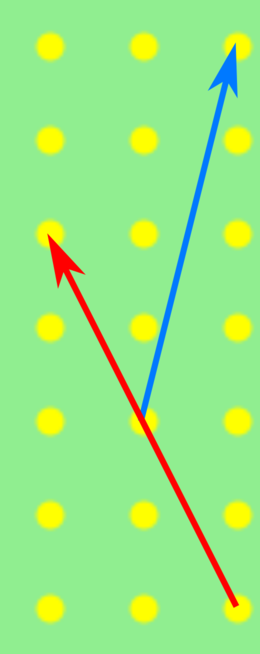
\includegraphics[scale=0.183, natwidth=288, natheight=657]{cropped.png}
  \caption{Collision}
  \label{fig:collision}
  The player with the blue movement line has the priority.
  \vspace{-1cm}
\end{wrapfigure}

\subsection{Collisions and Priorities}
When no course outs take place and movement lines of two players touch
or intersect, a {\em collision} takes place.

On a collision, the player with the {\em priority} will move to its
planned position, but one without the priority will be made to stay in
the same position.  The acceleration is applied the same as when no
collisions take place.

The player with the smaller $y$-coordinate of its position has the
priority.  When two players have the same $y$-coordinate, one with the
smaller $x$-coordinate has the priority.  An exception is when the
movement line of a player reaches or passes the opponent's original
position.  In this case, the priority is given to the opponent.

When movement lines of both players reaches or passes the opponents'
position, both lose the priority and cannot move at that step.

\subsection{Goal Time}
When a player at $(x, y)$ at step $s$ moves to $(x', y')$, and $y'\ge
l$ ($l$ is the course length) holds, that player finishes the race.
The goal time of the player is $s + (l-y)/(y'-y).$

A player that committed a course out or made a collision without
priority is stopped, and even if its planned position has
$y$-coordinate greater than or equal to the course length, the player
does not finish the race.

\section{Behavior of AI's}

The AI receives information related to the race as a whole at its
initiation, and responds with an acknowledgment of receiving it.  At
each step, it receives the race state information and responds with an
acceleration instruction.

The input of the AI is a sequence of decimal integers, separated by
blank spaces or newlines.  Negative values are prefixed with a minus
sign.  The initial game information and game state information at each
step end with a newline.

AI should respond sequences of decimal integers, separated by blank
spaces or newlines.  Negative values should be prefixed with a minus
sign.  {\bf A newline should be placed at the ends of responses.}

\subsection{Initial Input}
At initiation, AI receives the following input items in this order.
\begin{description}
\item[Remaining Time($t_{given}$)] The remaining time usable in this race in
  microseconds as an integer.
\item[Step Limit($s_{max}$)] The limit of number of steps to finish as an integer.
\item[Course Size] The width($w$) and length($l$) of the race course as two integers.
\item[Vision Limit($d$)] The depth of the field of vision as an integer
  $d.$ When the player is at $(x, y),$ information of the opponent and
  obstacle points are given for those at $y$-coordinates between $y-d$
  and $y+d$, inclusive.
\end{description}

\makeatletter
\def\lst@visiblespace{$\color{Gray}{}_{
  \mbox{\kern.06em\vrule \@height.3ex}%
  \vbox{\hrule \@width.3em}%
  \hbox{\vrule \@height.3ex}}$}
\makeatother

\lstset{
  basicstyle=\ttfamily,
  frame = single,
  showspaces = true,
  escapeinside={<@}{@>},
  mathescape
}

\subsection{Initial Input Format}
\begin{lstlisting}
$t_{given}$<@\tiny{\keys{\return}}@>
$s_{max}$<@\tiny{\keys{\return}}@>
$w$ $l$<@\tiny{\keys{\return}}@>
$d$<@\tiny{\keys{\return}}@>
\end{lstlisting}

\subsection{Initial Output}
A player AI should respond with an integer $0$ to acknowledge that its
initiation is done.

\begin{lstlisting}
0<@\tiny{\keys{\return}}@>
\end{lstlisting}

\subsection{Per Step Input}
At each step, AI receives the following items in this order.
\begin{description}
\item[Step($s$)] The current step number as a single integer.
\item[Remaining Time($t_{left}$)] The remaining time usable in this race in
  microseconds as an integer.
\item[Player's State] The $x$- and $y$-coordinates of the position and
  the $x$ and $y$ components the velocity of the player the AI is
  controlling, as four integers.
\item[Opponent's State] The $x$- and $y$-coordinates of the position and
  the $x$ and $y$ components the velocity of the opponent player, as
  four integers.  When the opponent player is out of the vision field,
  $-1$ is indicated for the $y$-coordinate of the position and $0$ for
  the remaining.
\item[Obstacle Points] Information on whether or not grid points in
  the vision field are obstacle points or not.  It consists of
  $(2\times d+1)\times w$ integers.  For every $y$ in the range
  $y_{\rm min} \le y \le y_{\rm max},$ $w$ integers $o_{0,y}, o_{1,y},
  \ldots, o_{w-1,y}$ are given.  $o_{x,y}$ being $1$ means that the
  grid point with its coordinates $(x,y)$ is an obstacle point, and
  $0$ means that it is not.  $1$ is given for grid points out of the
  rourse, that are, those with $y<0$.

\end{description}


\subsection{Per Step Input Format}
\begin{lstlisting}
$s$<@\tiny{\keys{\return}}@>
$t_{left}$<@\tiny{\keys{\return}}@>
$x$ $y$ $v_x$ $v_y$<@\tiny{\keys{\return}}@>
$x_e$ $x_e$ $v_{x_e}$ $v_{y_e}$<@\tiny{\keys{\return}}@>
$o_{0,y-d}$ $o_{1,y-d}$ ... $o_{w-1,y-d}$<@\tiny{\keys{\return}}@>
$o_{0,y-d+1}$ $o_{1,y-d+1}$ ... $o_{w-1,y-d+1}$<@\tiny{\keys{\return}}@>
...
$o_{0,y+d}$ $o_{1,y+d}$ ... $o_{w-1,y+d}$<@\tiny{\keys{\return}}@>
\end{lstlisting}

\subsection{Per Step Output}
The player AI should output $x$- and $y$-components of the
acceleration at the clock with two integers $a_{\rm x}$ and $a_{\rm
  y}$ as two integers.

\begin{lstlisting}
$a_{\rm x}$ $a_{\rm y}$<@\tiny{\keys{\return}}@>
\end{lstlisting}

\subsection{Sample Input}


\begin{minipage}[t]{.6\textwidth}

右に実際の入力例を示す.これは初期化から2ステップまでの入力となっている.

初期化時の入力について,考慮時間,制限ステップ数,コースの幅,
長さと視界がそれぞれ 20000, 100, 15, 100, 8
となっていることが分かる.

この入力を受け取ったらプレイヤーは0と改行をを出力しなければならない.

以降はステップごとの入力情報になるが,まず最初のステップについて
現在のステップと残り考慮時間がそれぞれ 0, 19981
となっていることが確認できる.このAIは初期化時に 19 [\si{\micro \second}] だけかかり,
残り 19981 [\si{\micro \second}] 残されているようだ.

次の2行は自プレイヤと相手プレイヤの状態が示されており,
このAIの現在の位置は $x = 5, y = 0$ で
速度は$x$軸方向$y$軸方向ともに0となっている.

次に続く17行($\text{視界:}8 \times 2 + 1$)は視界内の格子点が障害点か否かを示している.
$y < 0$におけるすべての格子点が障害点になることが分かる.
前方には中央に障害物が集中しているようだ.

この入力を受けたら,加速度$(a_x, a_y)$を出力する必要がある.
すると,また次のステップの入力が与えられる.
先ほどと同様の入力形式となっているが,どうやらこのAIは前ターンの加速度として
$(-1, 1)$を出力したようだ.

\end{minipage}
 \hfill
\begin{minipage}[t]{.3\textwidth}
\begin{lstlisting}[aboveskip = -1.4\medskipamount, showspaces = false, basicstyle = \tiny, literate = {-}{-}1]
20000
100
15 100
8
0
19981
5 0 0 0
9 0 0 0
1 1 1 1 1 1 1 1 1 1 1 1 1 1 1
1 1 1 1 1 1 1 1 1 1 1 1 1 1 1
1 1 1 1 1 1 1 1 1 1 1 1 1 1 1
1 1 1 1 1 1 1 1 1 1 1 1 1 1 1
1 1 1 1 1 1 1 1 1 1 1 1 1 1 1
1 1 1 1 1 1 1 1 1 1 1 1 1 1 1
1 1 1 1 1 1 1 1 1 1 1 1 1 1 1
1 1 1 1 1 1 1 1 1 1 1 1 1 1 1
0 0 0 0 0 0 0 0 0 0 0 0 0 0 0
0 0 0 0 0 0 0 0 0 0 0 0 0 0 0
0 0 0 0 0 0 0 1 0 0 0 0 0 0 0
0 0 0 0 0 0 0 1 0 0 0 0 0 0 0
0 0 0 0 0 0 1 1 0 0 0 0 0 0 0
0 0 0 0 0 0 1 1 1 0 0 0 0 0 0
0 0 0 0 0 1 1 1 1 0 0 0 0 0 0
0 0 0 0 0 1 1 1 1 0 0 0 0 0 0
0 0 0 0 1 1 1 1 1 1 0 0 0 0 0
1
19955
4 1 -1 1
8 1 -1 1
1 1 1 1 1 1 1 1 1 1 1 1 1 1 1
1 1 1 1 1 1 1 1 1 1 1 1 1 1 1
1 1 1 1 1 1 1 1 1 1 1 1 1 1 1
1 1 1 1 1 1 1 1 1 1 1 1 1 1 1
1 1 1 1 1 1 1 1 1 1 1 1 1 1 1
1 1 1 1 1 1 1 1 1 1 1 1 1 1 1
1 1 1 1 1 1 1 1 1 1 1 1 1 1 1
0 0 0 0 0 0 0 0 0 0 0 0 0 0 0
0 0 0 0 0 0 0 0 0 0 0 0 0 0 0
0 0 0 0 0 0 0 1 0 0 0 0 0 0 0
0 0 0 0 0 0 0 1 0 0 0 0 0 0 0
0 0 0 0 0 0 1 1 0 0 0 0 0 0 0
0 0 0 0 0 0 1 1 1 0 0 0 0 0 0
0 0 0 0 0 1 1 1 1 0 0 0 0 0 0
0 0 0 0 0 1 1 1 1 0 0 0 0 0 0
0 0 0 0 1 1 1 1 1 1 0 0 0 0 0
0 0 0 1 1 1 1 1 1 1 0 0 0 0 0
\end{lstlisting}
\end{minipage}

\subsection{Memory Duration}
At each step, the game management system suspends the execution of AI
when receiving its output has been completed, and resumes it after
giving per step information.  Thus AI cannot continue its computation
between steps but its execution context, including variable values,
are kept during one whole race.

For each race, the game management system initiates AI from scratch in
an environment in which file I/O and network accesses are disabled.
Thus, AI cannot pass information between multiple races.

\end{document}
